\section{Method of Moments}

\subsection{Discretization}
Starting from the EFIE, we expand the unknown current distribution $\vec{J}(\vecr)$ into a series of basis functions:
\begin{equation}
	\vec{J}(\vecr) = \sum_{n = 1}^{N} I_n \vec{f}_n(\vecr),
	\label{eq:j_exp}
\end{equation}
where $I_n$ are the unknown coefficients representing the current, and $\vec{f}_n(\vecr)$ are the vector basis functions. Many choices of basis are possible, but we will use the triangular basis functions shown in Figure~\ref{fig:mom_basis}. The orientation of the basis vectors $\hat{\vec{a}}_m$ is further discussed in Section~\ref{sec:mom_bc}.
\begin{figure}[!ht]
	\centering
	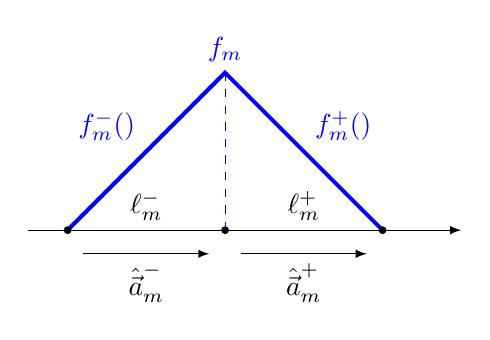
\begin{tikzpicture}[> = latex]
	\draw[->] (-0.5, 0) -- (5, 0);	
	
	\draw[blue, line width=0.5mm] (0, 0) -- node[above left] {$f_m^{-}(\vecr)$} (2, 2) node[above] {$f_m$} -- node[above right] {$f_m^{+}(\vecr)$} (4, 0);
	\draw[blue, dashed] (2, 0) -- (2, 2);
	\node[fill = black, circle, inner sep=0pt, minimum size = 1mm] at (0, 0) {};
	\node[fill = black, circle, inner sep=0pt, minimum size = 1mm] at (2, 0) {};
	\node[fill = black, circle, inner sep=0pt, minimum size = 1mm] at (4, 0) {};
	
	\draw (1, 0) node[above] {$\ell_m^{-}$};
	\draw (3, 0) node[above] {$\ell_m^{+}$};
	
	\draw[->] (0.2, -0.3) -- node[below] {$\hat{\vec{a}}_m^{-}$} (1.8, -0.3);
	\draw[->] (2.2, -0.3) -- node[below] {$\hat{\vec{a}}_m^{+}$} (3.8, -0.3);
\end{tikzpicture}
	\caption{Triangular basis function}
	\label{fig:mom_basis}
\end{figure}

Substituting (\ref{eq:j_exp}) into the EFIE, the $\oL$ operator now operates on the (known) basis functions.
\begin{equation}
	\vec{E}(\vecr) = j\omega\mu \sum_{n = 1}^{N} I_n (\oL \vec{f}_n)(\vecr)
	\label{eq:efie_exp}
\end{equation}
Next, we can test (\ref{eq:efie_exp}) with the same basis functions $\vec{f}_m(\vecr)$ with $m = 1, \dots, N$.
\begin{equation}
	\langle \vec{f}_m, \vec{E} \rangle = j\omega\mu \sum_{n = 1}^{N} I_n \langle \vec{f}_m, \oL \vec{f}_n \rangle \qquad m = 1, \dots, N
\end{equation}
This results in a dense, square $N \times N$ system of equations.
\begin{equation}
	\begin{Bmatrix}
		V
	\end{Bmatrix} = \begin{bmatrix}
		Z
	\end{bmatrix} \begin{Bmatrix}
		I
	\end{Bmatrix},
	\label{eq:system}
\end{equation}
with
\begin{align*}
	V_m & = \int_{f_m} \vec{f}_m(\vecr) \cdot \vec{E}(\vecr) d\vecr \\
	Z_{mn} & = j\omega\mu \int_{f_m} \int_{f_n} \vec{f}_m(\vecr) \cdot \vec{f}_n(\vecrp) G_k(\vecr, \vecrp) d\vecrp d\vecr \\
	 & - \frac{1}{j\omega} \int_{f_m} \int_{f_n} \nabla \cdot \vec{f}_m(\vecr) \nabla^\prime \cdot \vec{f}_n(\vecrp) G_k(\vecr, \vecrp) d\vecrp d\vecr
\end{align*}
For ease of notation and to clarify the physical role each integral term plays, we redefine the impedance contribution in terms of the vector potential $\vec{A}$ and the scalar potential $\Phi$.
\begin{equation}
	Z_{mn} = j\omega\mu A_{mn} - \frac{j}{\omega\varepsilon} \Phi_{mn} = j k \eta_0 \left(A_{mn} - \frac{1}{k^2} \Phi_{mn} \right),
\end{equation}
where
\begin{align}
	A_{mn} & = \int_{f_m} \int_{f_n} \vec{f}_m(\vecr) \cdot \vec{f}_n(\vecrp) G_k(\vecr, \vecrp) d\vecrp d\vecr \label{eq:Amn} \\
	\Phi_{mn} & = \int_{f_m} \int_{f_n} \nabla \cdot \vec{f}_m(\vecr) \nabla^\prime \cdot \vec{f}_n(\vecrp) G_k(\vecr, \vecrp) d\vecrp d\vecr \label{eq:Pmn}
\end{align}

\subsubsection{Quadrature}

\begin{equation}
	\int_{-1}^{+1} I(x) dx \approx \sum_{p = 1}^{M} w_p I(x_p),
\end{equation}
with quadrature weights $w_p$ and quadrature points $x_p$. In the Julia code, the Gauss-Legendre quadrature is used.

\subsubsection{Non-Self Terms}
The basis and testing functions are defined on (two-dimensional) segments of thin wire in three-dimensional space. Considering a pair of non-overlapping basis functions $n,m$, we can calculate the integrals numerically by applying a quadrature rule to both integrals. Because each shape function consists of two parts (for triangular basis functions), we can split the contributions into four parts.
\begin{align}
	A_{mn} & = A_{mn}^{++} + A_{mn}^{+-} + A_{mn}^{-+} + A_{mn}^{--} \label{eq:amn_nodal} \\
	\Phi_{mn} & = \Phi_{mn}^{++} + \Phi_{mn}^{+-} + \Phi_{mn}^{-+} + \Phi_{mn}^{--} \label{eq:pmn_nodal}
\end{align}
The contributions to the vector potential are derived from (\ref{eq:Amn}). The superscripts refer to the positive and negative elements belonging to the basis functions $m$ and $n$ as defined in Figure~\ref{fig:mom_basis2}.
\begin{figure}[b]
	\centering
	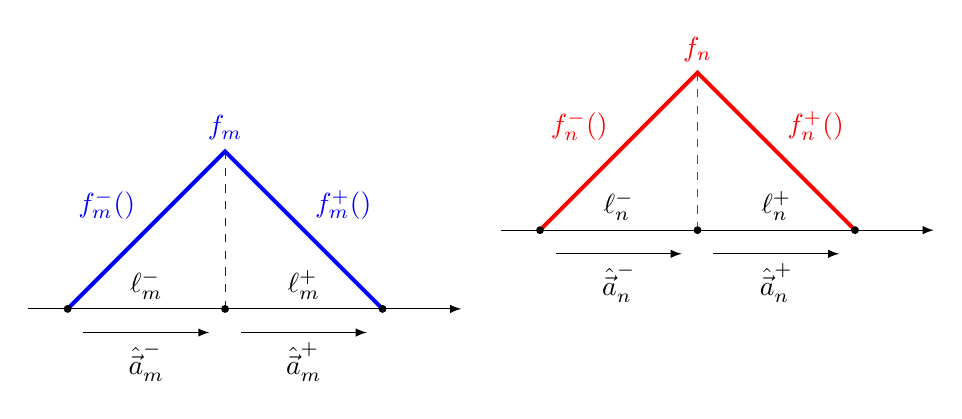
\begin{tikzpicture}[> = latex]
	\draw[->] (-0.5, 0) -- (5, 0);	
	
	\draw[blue, line width=0.5mm] (0, 0) -- node[above left] {$f_m^{-}(\vecr)$} (2, 2) node[above] {$f_m$} -- node[above right] {$f_m^{+}(\vecr)$} (4, 0);
	\draw[blue, dashed] (2, 0) -- (2, 2);
	\node[fill = black, circle, inner sep=0pt, minimum size = 1mm] at (0, 0) {};
	\node[fill = black, circle, inner sep=0pt, minimum size = 1mm] at (2, 0) {};
	\node[fill = black, circle, inner sep=0pt, minimum size = 1mm] at (4, 0) {};
	
	\draw (1, 0) node[above] {$\ell_m^{-}$};
	\draw (3, 0) node[above] {$\ell_m^{+}$};
	
	\draw[->] (0.2, -0.3) -- node[below] {$\hat{\vec{a}}_m^{-}$} (1.8, -0.3);
	\draw[->] (2.2, -0.3) -- node[below] {$\hat{\vec{a}}_m^{+}$} (3.8, -0.3);
	
	
	\draw[->] (5.5, 1) -- (11, 1);	
	
	\draw[red, line width=0.5mm] (6, 1) -- node[above left] {$f_n^{-}(\vecr)$} (8, 3) node[above] {$f_n$} -- node[above right] {$f_n^{+}(\vecr)$} (10, 1);
	\draw[red, dashed] (8, 1) -- (8, 3);
	\node[fill = black, circle, inner sep=0pt, minimum size = 1mm] at (6, 1) {};
	\node[fill = black, circle, inner sep=0pt, minimum size = 1mm] at (8, 1) {};
	\node[fill = black, circle, inner sep=0pt, minimum size = 1mm] at (10, 1) {};
	
	\draw (7, 1) node[above] {$\ell_n^{-}$};
	\draw (9, 1) node[above] {$\ell_n^{+}$};
	
	\draw[->] (6.2, 0.7) -- node[below] {$\hat{\vec{a}}_n^{-}$} (7.8, 0.7);
	\draw[->] (8.2, 0.7) -- node[below] {$\hat{\vec{a}}_n^{+}$} (9.8, 0.7);
\end{tikzpicture}
	\caption{Definition of (non-overlapping) basis functions.}
	\label{fig:mom_basis2}
\end{figure}
\begin{align*}
	A_{mn}^{++} & = \hat{\vec{a}}_m^{+} \cdot \hat{\vec{a}}_n^{+} \frac{\ell_m^{+} \ell_n^{+}}{4} \sum_{p = 1}^M \sum_{q = 1}^M w_p w_q f_m(\vec{r}_p^{+}) f_n(\vec{r}_q^{+}) G(\vec{r}_p^{+}, \vec{r}_q^{+}) \\
	A_{mn}^{+-} & = \hat{\vec{a}}_m^{+} \cdot \hat{\vec{a}}_n^{-} \frac{\ell_m^{+} \ell_n^{-}}{4} \sum_{p = 1}^M \sum_{q = 1}^M w_p w_q f_m(\vec{r}_p^{+}) f_n(\vec{r}_q^{-}) G(\vec{r}_p^{+}, \vec{r}_q^{-}) \\
	A_{mn}^{-+} & = \hat{\vec{a}}_m^{-} \cdot \hat{\vec{a}}_n^{+} \frac{\ell_m^{-} \ell_n^{+}}{4} \sum_{p = 1}^M \sum_{q = 1}^M w_p w_q f_m(\vec{r}_p^{-}) f_n(\vec{r}_q^{+}) G(\vec{r}_p^{-}, \vec{r}_q^{+}) \\
	A_{mn}^{--} & = \hat{\vec{a}}_m^{-} \cdot \hat{\vec{a}}_n^{-} \frac{\ell_m^{-} \ell_n^{-}}{4} \sum_{p = 1}^M \sum_{q = 1}^M w_p w_q f_m(\vec{r}_p^{-}) f_n(\vec{r}_q^{-}) G(\vec{r}_p^{-}, \vec{r}_q^{-})
\end{align*}
Similarly, for the scalar potential contributions. Here, we can pre-calculate the divergence of the basis functions, which is constant over the element (for triangular basis functions).
\begin{align}
	\nabla \cdot \vec{f}_m^{+}(\vecr) & = \frac{-1}{\ell_m^+} \qquad \vecr \in \operatorname{supp}(f_m^+) \\
	\nabla \cdot \vec{f}_m^{-}(\vecr) & = \frac{+1}{\ell_m^-} \qquad \vecr \in \operatorname{supp}(f_m^-)
\end{align}
Therefore, the scalar potential terms become
\begin{align*}
	\Phi_{mn}^{++} & = \frac{-1}{\ell_{m}^{+}} \frac{-1}{\ell_{m}^{+}} \frac{\ell_m^{+} \ell_n^{+}}{4} \sum_{p = 1}^M \sum_{q = 1}^M w_p w_q G(\vec{r}_p^{+}, \vec{r}_q^{+}) \\
	& = \frac{1}{4} \sum_{p = 1}^M \sum_{q = 1}^M w_p w_q G(\vec{r}_p^{+}, \vec{r}_q^{+}) \\
	\Phi_{mn}^{+-} & = -\frac{1}{4} \sum_{p = 1}^M \sum_{q = 1}^M w_p w_q G(\vec{r}_p^{+}, \vec{r}_q^{-}) \\
	\Phi_{mn}^{-+} & = -\frac{1}{4} \sum_{p = 1}^M \sum_{q = 1}^M w_p w_q G(\vec{r}_p^{-}, \vec{r}_q^{+}) \\
	\Phi_{mn}^{--} & = \frac{1}{4} \sum_{p = 1}^M \sum_{q = 1}^M w_p w_q G(\vec{r}_p^{-}, \vec{r}_q^{-})
\end{align*}

\subsubsection{Self Terms}
If the basis functions $n, m$ overlap (see Figure~\ref{fig:mom_basis3}), then we must treat the singularity that arises in the integral of the Green's function. We can do this by evaluating the inner integral analytically and the outer integral numerically using an $M$-point quadrature rule. Assume that the singularity is in the $++$ direction (only possible when $m = n$). For the vector potential term,
\begin{figure}[t]
	\centering
	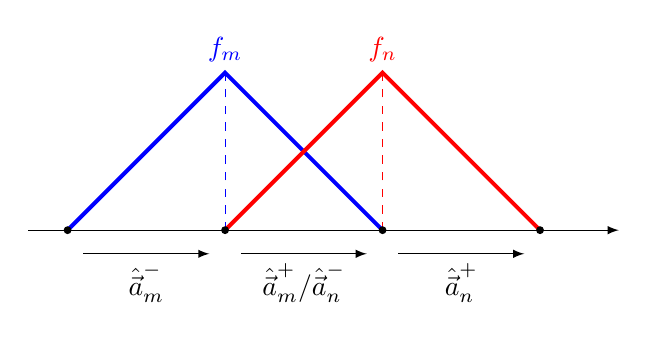
\begin{tikzpicture}[> = latex]
	\draw[->] (-0.5, 0) -- (7, 0);	
	
	\draw[blue, line width=0.5mm] (0, 0) -- (2, 2) node[above] {$f_m$} -- (4, 0);
	\draw[red, line width=0.5mm] (2, 0) -- (4, 2) node[above] {$f_n$} -- (6, 0);
	\draw[blue, dashed] (2, 0) -- (2, 2);
	\draw[red, dashed] (4, 0) -- (4, 2);
	\node[fill = black, circle, inner sep=0pt, minimum size = 1mm] at (0, 0) {};
	\node[fill = black, circle, inner sep=0pt, minimum size = 1mm] at (2, 0) {};
	\node[fill = black, circle, inner sep=0pt, minimum size = 1mm] at (4, 0) {};
	\node[fill = black, circle, inner sep=0pt, minimum size = 1mm] at (6, 0) {};
	
	\draw[->] (0.2, -0.3) -- node[below] {$\hat{\vec{a}}_m^{-}$} (1.8, -0.3);
	\draw[->] (2.2, -0.3) -- node[below] {$\hat{\vec{a}}_m^{+}$/$\hat{\vec{a}}_n^{-}$} (3.8, -0.3);
	\draw[->] (4.2, -0.3) -- node[below] {$\hat{\vec{a}}_n^{+}$} (5.8, -0.3);
\end{tikzpicture}
	\caption{Definition of (overlapping) basis functions.}
	\label{fig:mom_basis3}
\end{figure}
\begin{align*}
	A_{mn}^{++} & = \hat{\vec{a}}_m^{+} \cdot \hat{\vec{a}}_n^{+} \frac{\ell_m^+}{2} \sum_{p = 1}^M w_p f_m(\vec{r}_p^+) \int_{f_n} f_n(\vecrp) G(\vecr_p^+, \vecrp) d\vecrp \\
	& = \hat{\vec{a}}_m^{+} \cdot \hat{\vec{a}}_n^{+} \frac{\ell_m^+}{2} \sum_{p = 1}^M w_p f_m(\vec{r}_p^+) S_1(\vecr_p^+)
\end{align*}
And for the scalar potential term,
\begin{equation*}
	\Phi_{mn}^{++} = \frac{\ell_m^+}{2} \sum_{p = 1}^M w_p \frac{1}{\ell_m^+ \ell_n^+} \int_{f_n} G(\vecr_p^+, \vecrp) d\vecrp = \frac{\ell_m^+}{2} \sum_{p = 1}^M w_p S_2(\vecr_p^+)
\end{equation*}
where we define $S_1$ and $S_2$ as follows
\begin{align}
	S_1(\vecr) & = \int_{f_n} f_n(\vecrp) G(\vecr, \vecrp) d\vecrp \\
	S_2(\vecr) & = \frac{1}{s^2} \int_{f_n} G(\vecr, \vecrp) d\vecrp
\end{align}
where $s$ is the length of the segment containing the singularity. 

\subsubsection{Thin-Wire Approximation}
We apply the thin-wire approximation to find an analytical expression for the integrals $S_1$ and $S_2$. That is, we assume that the one-dimensional elements are, in fact, wires with a radius $a$, which is small compared to the length of the element $\ell_n$ and the wavelength $\lambda$. We redefine the distance between $\vecr$ and $\vecrp$ as
\begin{equation*}
	|\vecr - \vecrp| = \sqrt{(r - r^\prime)^2 + a^2}
\end{equation*}
Then, the two integrals can be evaluated analytically. The detailed derivation is presented in Gibson, 2021.
\begin{equation}
	\begin{aligned}
		S_1(x, s) & = \frac{1}{4\pi} \left[ \frac{1}{s} \sqrt{a^2 + (x - s)^2} - \frac{1}{s} \sqrt{a^2 + x^2} \right. \\
		 & + \left. \frac{x}{s} \frac{\log\left( x + \sqrt{x^2 + a^2} \right)}{x - s + \sqrt{a^2 + (x - s)^2}} - \frac{j k s}{2} \right]
	\end{aligned}
\end{equation}

\begin{equation}
	S_2(x, s) = \frac{1}{4\pi s^2} \left[ \frac{\log\left( x + \sqrt{x^2 + a^2} \right)}{x - s + \sqrt{a^2 + (x - s)^2}} - j k s\right]
\end{equation}

\subsection{Practical Element-Wise Matrix Assembly}
To assemble the system matrix equation (\ref{eq:system}), we loop over all pairs of nodal basis functions and calculate the contributions of each part using (\ref{eq:amn_nodal}), (\ref{eq:pmn_nodal}). A more practical method of matrix assembly is to loop over all pairs of elements, each with pre-defined basis functions (see Figure~\ref{fig:mom_basis4}).
\begin{figure}[b]
	\centering
	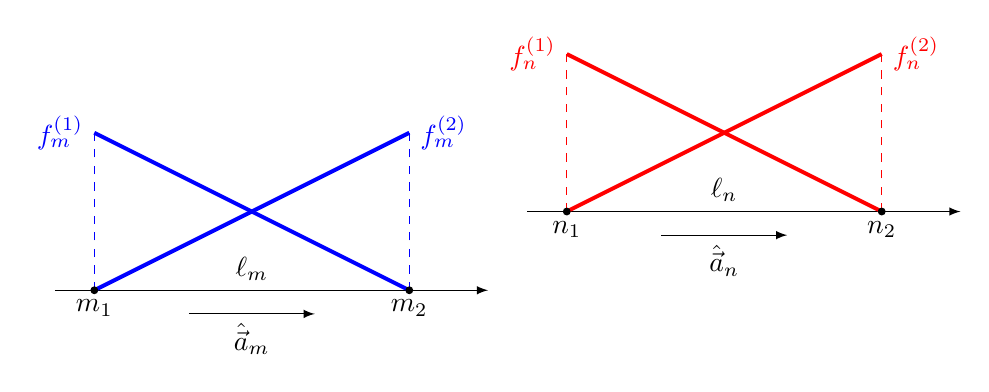
\begin{tikzpicture}[> = latex]
	\draw[->] (-0.5, 0) -- (5, 0);	
	
	\draw[blue, line width=0.5mm] (0, 2) node[left] {$f_m^{(1)}$} -- (4, 0);
	\draw[blue, line width=0.5mm] (0, 0) -- (4, 2) node[right] {$f_m^{(2)}$};
	
	\draw[blue, dashed] (0, 0) -- (0, 2);
	\draw[blue, dashed] (4, 0) -- (4, 2);
	\draw (0, 0) node[fill = black, circle, inner sep=0pt, minimum size = 1mm] {} node[below] {$m_1$};
	\draw (4, 0) node[fill = black, circle, inner sep=0pt, minimum size = 1mm] {} node[below] {$m_2$};
	
	\draw (2, 0) node[above] {$\ell_m$};
	
	\draw[->] (1.2, -0.3) -- node[below] {$\hat{\vec{a}}_m$} (2.8, -0.3);
	
	\draw[->] (5.5, 1) -- (11, 1);	
	
	\draw[red, line width=0.5mm] (6, 3) node[left] {$f_n^{(1)}$} -- (10, 1);
	\draw[red, line width=0.5mm] (6, 1) -- (10, 3) node[right] {$f_n^{(2)}$};
	\draw[red, dashed] (6, 1) -- (6, 3);
	\draw[red, dashed] (10, 1) -- (10, 3);
	\draw (6, 1) node[fill = black, circle, inner sep=0pt, minimum size = 1mm] {} node[below] {$n_1$};
	\draw (10, 1) node[fill = black, circle, inner sep=0pt, minimum size = 1mm] {} node[below] {$n_2$};
	
	\draw (8, 1) node[above] {$\ell_n$};
	
	\draw[->] (7.2, 0.7) -- node[below] {$\hat{\vec{a}}_n$} (8.8, 0.7);
\end{tikzpicture}
	\caption{Definition of element-local basis functions.}
	\label{fig:mom_basis4}
\end{figure}

Each element contributes to four locations in the system matrix ($[m_1, n_1]$, $[m_1, n_2]$, $[m_2, n_1]$, $[m_2, n_2]$), allowing the local contribution to be written conveniently as a $2 \times 2$ matrix. This way of constructing the local contribution is very similar to the way this is done in the finite element method.
\begin{align}
	A_{mn} & = \hat{\vec{a}}_m \cdot \hat{\vec{a}}_n \frac{\ell_m \ell_n}{4} \sum_{p = 1}^M \sum_{q = 1}^M w_p w_q \begin{bmatrix}
		f_{m,p}^{(1)} f_{n,q}^{(1)} & f_{m,p}^{(1)} f_{n,q}^{(2)} \\
		f_{m,p}^{(2)} f_{n,q}^{(1)} & f_{m,p}^{(2)} f_{n,q}^{(2)}
	\end{bmatrix} G(\vec{r}_p, \vec{r}_q) \\
	\Phi_{mn} & = \frac{1}{4} \sum_{p = 1}^M \sum_{q = 1}^M w_p w_q \begin{bmatrix}
		+1 & -1 \\ -1 & +1
	\end{bmatrix} G(\vec{r}_p, \vec{r}_q)
\end{align}
where $f_{m,p}^{(1)}$ is basis function $f_m^{(1)}$, evaluated at $\vecr_p$, etc. 

It is now very easy to determine whether the self or non-self terms must be used since there is only an overlap of basis functions when elements $m$ and $n$ are the same, i.e., $m = n$. The self-terms become
\begin{align}
	A_{mm} & = \frac{\ell_m}{2} \sum_{p = 1}^M w_p \begin{bmatrix}
		f_{m,p}^{(1)} & f_{m,p}^{(1)} \\
		f_{m,p}^{(2)} & f_{m,p}^{(2)}
	\end{bmatrix} S_1(\vecr_p) \\
	\Phi_{mm} & = \frac{\ell_m}{2} \sum_{p = 1}^M w_p \begin{bmatrix}
		+1 & -1 \\ -1 & +1
	\end{bmatrix} S_2(\vecr_p)
\end{align}

\subsection{Boundary Conditions}
\label{sec:mom_bc}
Two boundary conditions arise from the equation of charge conservation:
\begin{enumerate}
	\item The basis vectors $\vec{a}_n$ should be oriented such that (\ref{eq:charge_cons}) holds at every node.
	\item A condition $I = 0$ must be imposed on the end-points of every segment, as this is the only way to enforce (\ref{eq:charge_cons}).
\end{enumerate}
\begin{equation}
	\nabla \cdot \vec{J} = 0
	\label{eq:charge_cons}	
\end{equation}

\subsection{Post-processing}

\subsubsection{Antenna impedance}
To calculate the impedance seen by a source embedded in segment $e$, with nodes $n_1, n_2$, we make use of the current coefficient vector $\begin{Bmatrix}
	I
\end{Bmatrix}$. The impedance is defined as
\begin{equation}
	Z = \frac{V_{src}}{I_{src}},
\end{equation}
where $V_{src}$ is the known source voltage and $I_{src}$ is the solved current averaged over segment $e$:
\begin{equation*}
	I_{src} = \frac{1}{2}\left( I[n_1] + I[n_2] \right)
\end{equation*}

\subsubsection{Far-field radiation}
The far-field radiation pattern can also be derived from the solved current vector. The EFIE can be simplified by assuming that the $\nicefrac{1}{r}$ are dominant and that higher-order terms have negligible amplitude in the far field.
\begin{equation}
	\vec{E}(\vecr) = -j\omega\mu \int \vec{J}(\vecrp) G_k(\vecr, \vecrp) d\vecrp
	\label{eq:ff_efie}
\end{equation}
This expression can be further simplified by considering that $\vecr \gg \vecrp$, such that
\begin{equation}
	|\vecr - \vecrp| = \left\{ \begin{array}{ll}
		r \quad & \text{for amplitude variations} \\
		r - \vecrp \cdot \hat{\vecr} \quad & \text{for phase variations}
	\end{array} \right.
	\label{eq:ff_approx}
\end{equation}
where $r = |\vecr|$ and $\hat{\vecr} = \nicefrac{\vecr}{|\vecr|}$. Applying (\ref{eq:ff_approx}) to (\ref{eq:ff_efie}) yields
\begin{equation}
	\vec{E}(\vecr) = j\omega\mu \frac{e^{-j k r}}{4\pi r} \int ((\hat{\vecr} \cdot \vec{J}(\vecrp)) \hat{\vecr} - \vec{J}(\vecrp)) e^{j k \vecrp \cdot \hat{\vecr}} d\vecrp
\end{equation}
Applying the same discretization procedure,
\begin{equation}
	\vec{E}(\vecr) = j\omega\mu \frac{e^{-j k r}}{4\pi r} \sum_{n = 1}^{N} I_n \int_{f_n} ((\hat{\vecr} \cdot \hat{\vec{a}}_n) \hat{\vecr} - \hat{\vec{a}}_n) f_n(\vecrp) e^{j k \vecrp \cdot \hat{\vecr}} d\vecrp
\end{equation}
The integral can be tackled using quadrature, and all the terms are known.